\section{Stroke Rendering}

\subsection{用三角形畫粗線}
\label{sec:stroke-geometry}

Outline 與 Filled 模式以 \lstinline|glLineWidth()| 搭配 OpenGL 線條繪製。線寬較小時不易察覺問題，但線寬增加到 25 px 時，矩形轉角會出現圖~\ref{fig:native-custom-stroke} 左側的缺角與突出。原因是 OpenGL 的寬線逐段獨立光柵化，線段兩端只會切成水平或垂直的邊，相鄰兩段在轉角處無法對齊。此外，OpenGL 無法設定轉角與端點樣式，最大線寬也由實作決定。因此 Advanced 模式改為自行將中心線展開成三角形，結果如同圖右側。

展開的基本單位是單一線段。對線段 $A\to B$，設線寬為 $w$、半線寬 $h=w/2$，其單位方向與法向量為
\[
    \vec u=\frac{B-A}{\norm{B-A}},\qquad \vec n=(-u_y,u_x).
\]
由於 Canvas 的 Y 軸向下，$\vec n$ 指向前進方向的右側，因此線段兩端的左右邊界點為
\[
    A_L=A-h\vec n,\quad A_R=A+h\vec n,\qquad
    B_L=B-h\vec n,\quad B_R=B+h\vec n.
\]
這四點圍成寬度為 $w$ 的四邊形，再拆成 $\triangle A_LA_RB_R$ 和 $\triangle A_LB_RB_L$ 兩個三角形交由 OpenGL 繪製。

然而折線的每個頂點同時屬於前後兩段，若各段分別使用 $B\pm h\vec n$，轉角仍無法對齊。因此程式先為每個頂點計算左右兩個「截面點」，再以相鄰頂點的截面點組成線身。截面點預設為上述邊界點，在轉角處依第~\ref{sec:line-join} 節的 Join 調整，在開放路徑的端點則依第~\ref{sec:line-cap} 節的 Cap 調整。長度為零的線段沒有方向，不產生線身，相關處理見第~\ref{sec:stroke-degenerate} 節。

\begin{figure}[htbp]
    \centering
    \begin{subfigure}[t]{.49\textwidth}
        \centering
        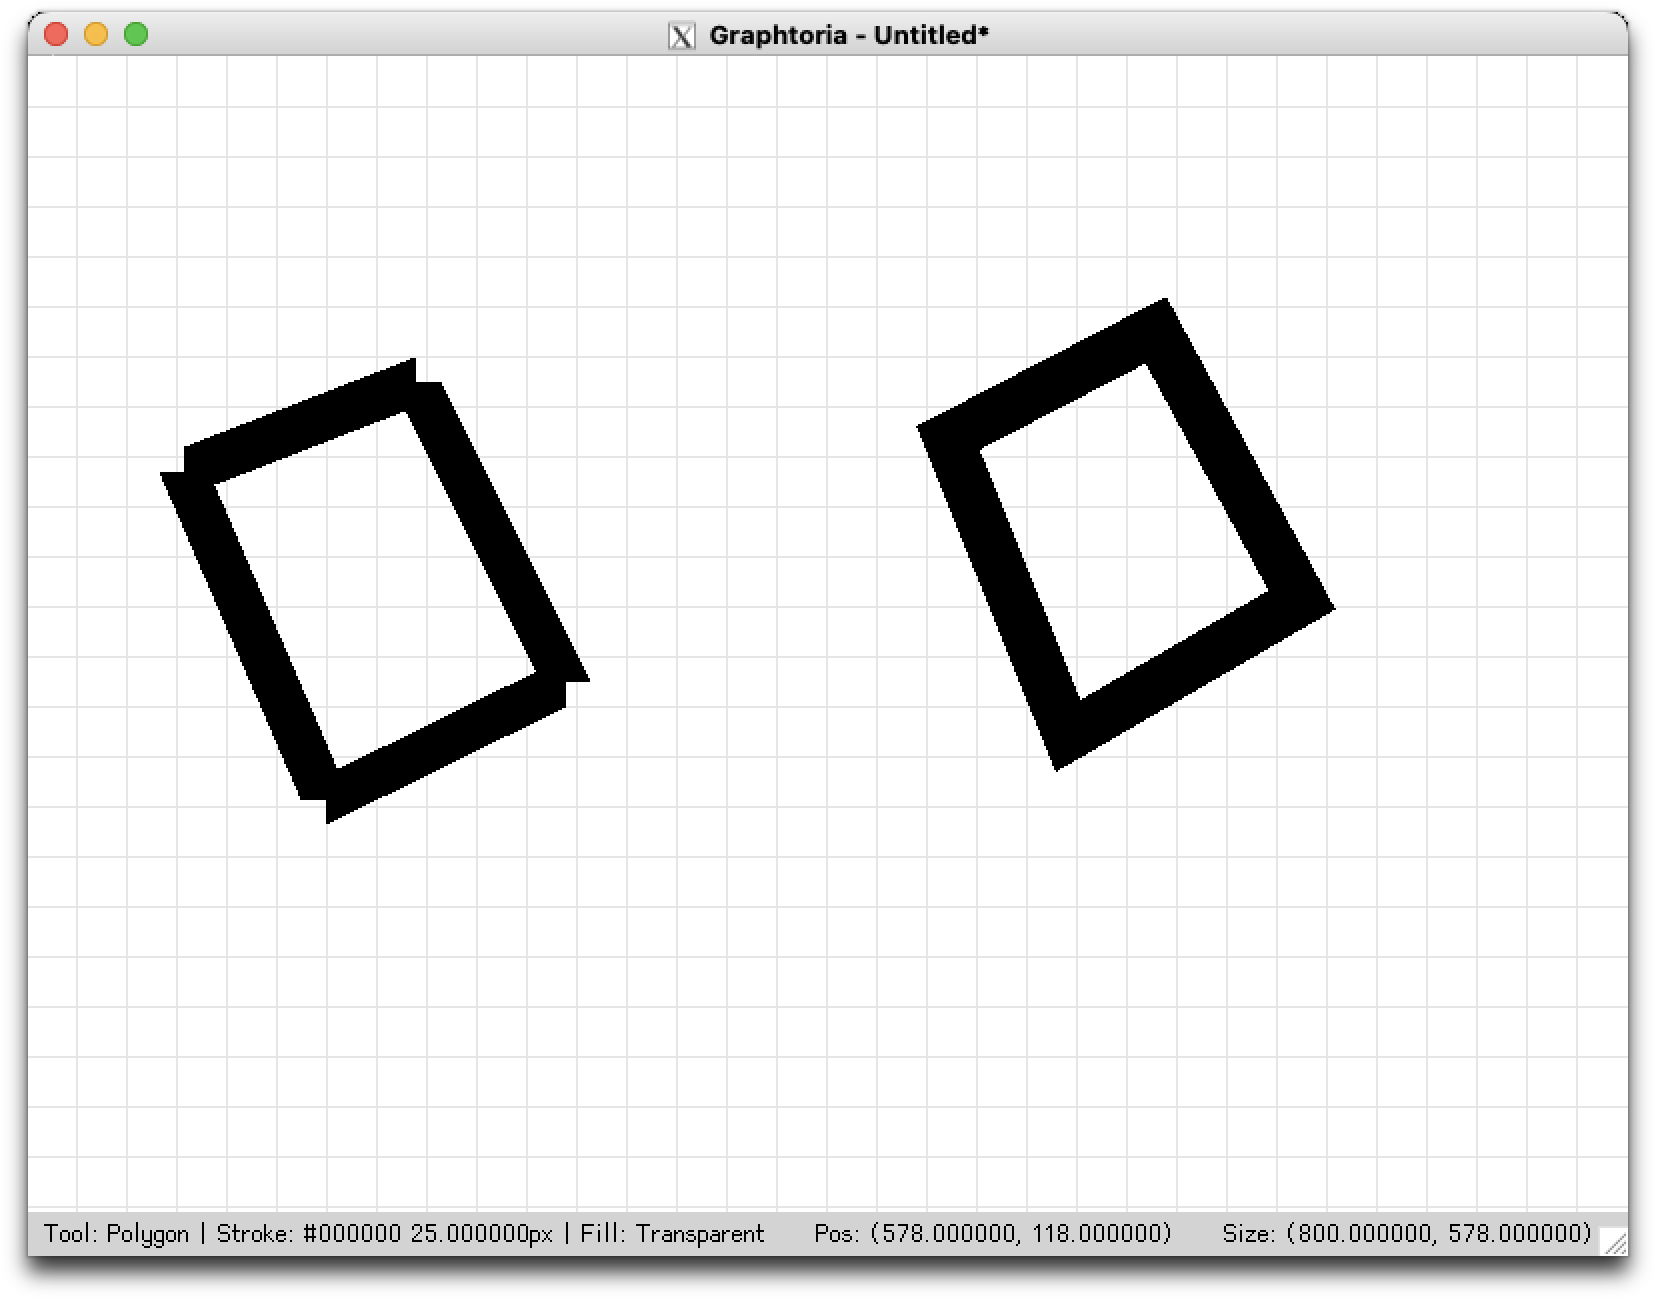
\includegraphics[width=\linewidth]{docs/figures/ch04_native-custom-stroke.png}
        \caption{OpenGL 粗線與自製 Stroke}
        \label{fig:native-custom-stroke}
    \end{subfigure}\hfill
    \begin{subfigure}[t]{.49\textwidth}
        \centering
        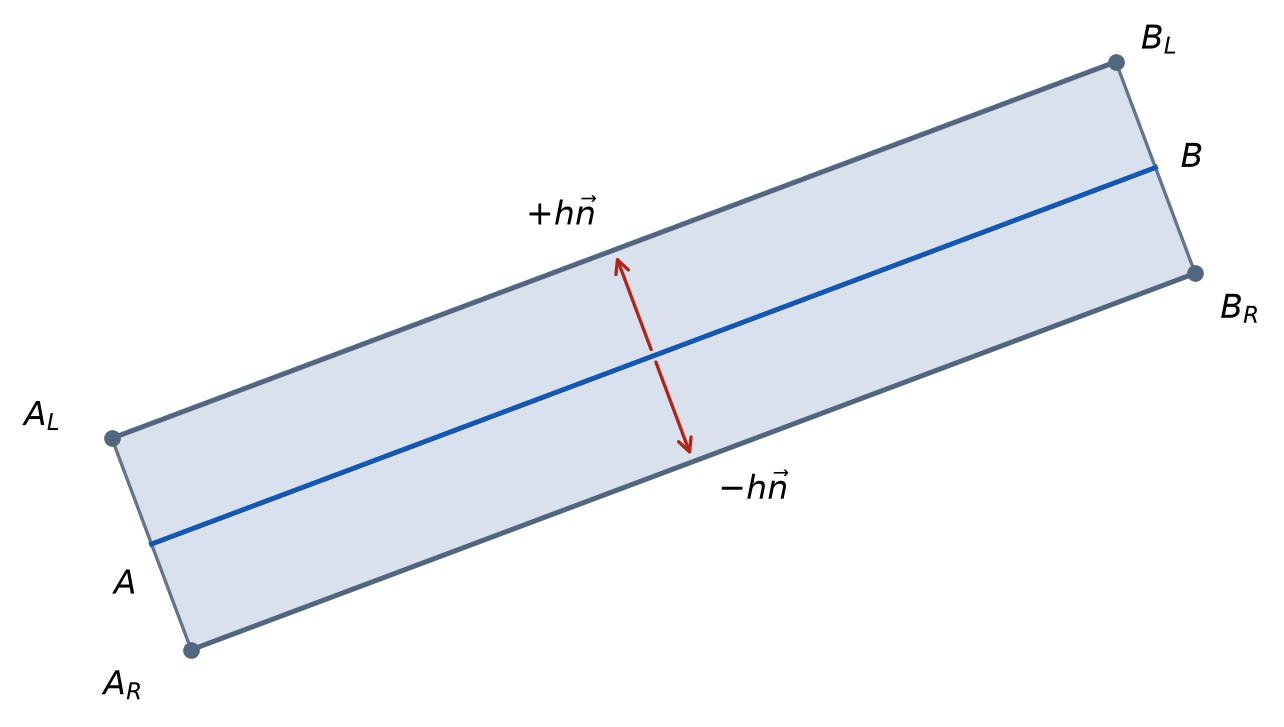
\includegraphics[width=\linewidth]{docs/figures/ch04_stroke-expansion.png}
        \caption{中心線向兩側展開}
        \label{fig:stroke-expansion}
    \end{subfigure}
    \caption{自行建立 Stroke Geometry 的原因與基本方法}
    \label{fig:stroke-overview}
\end{figure}

\subsection{Line Join}
\label{sec:line-join}

若每段僅依圖~\ref{fig:stroke-expansion} 各自展開，轉角外側會留下缺口，內側則互相重疊，因此每個頂點都需要另外處理。對每個頂點 $B$，取前一點 $A$ 與下一點 $C$，兩段的方向與法向量分別為
\[
    \vec u=\frac{B-A}{\norm{B-A}},\qquad
    \vec v=\frac{C-B}{\norm{C-B}},\qquad
    \vec n_0=(-u_y,u_x),\qquad
    \vec n_1=(-v_y,v_x).
\]
與第~\ref{sec:stroke-geometry} 節相同，$AB$ 的左、右邊界是中心線平移 $-h\vec n_0$ 與 $+h\vec n_0$ 所得的 offset line，$BC$ 亦同。

\paragraph{判斷內外側}
處理轉角前需先確定內側與外側。兩段的轉向由二維外積判斷：
\[
    c=\vec u\times\vec v=u_xv_y-u_yv_x.
\]
在 Y 軸向下的畫面上，$c>0$ 表示向右（順時針）轉，此時右側為內側、左側為外側；$c<0$ 時相反。$c$ 接近 $0$ 表示兩段幾乎平行或折返，於第~\ref{sec:stroke-degenerate} 節說明。

\paragraph{求 offset line 交點}
左右兩側分別求 $AB$ 與 $BC$ 兩條 offset line 的交點。將兩條直線表示為 $P+t\vec r$ 與 $Q+s\vec w$，當 $\vec r\times\vec w\ne0$ 時，交點為
\[
    t=\frac{(Q-P)\times\vec w}{\vec r\times\vec w},\qquad X=P+t\vec r.
\]
為避免除以接近零的數，當 $\abs{\vec r\times\vec w}\le\eps\,\norm{\vec r}\norm{\vec w}$ 時視為兩線平行，不使用交點。以下將內側交點記為 $X_{\text{in}}$、外側交點記為 $X_{\text{out}}$。

\paragraph{三種 Join}
三種 Join 的內側處理相同：兩段的內側邊界都收至 $X_{\text{in}}$，使線身在內側相接而不重疊。差別在於外側缺口的補法，效果如圖~\ref{fig:stroke-join}。
\begin{itemize}
    \item \textbf{Miter}：外側同樣收至 $X_{\text{out}}$，兩段線身在尖角處直接接合，不需額外三角形。轉角很尖時 $X_{\text{out}}$ 會遠離頂點，因此超過 Miter Limit 時改用 Bevel，推導見第~\ref{sec:miter-limit} 節與圖~\ref{fig:miter-limit}。
    \item \textbf{Bevel}：外側保留兩段各自在 $B$ 的截面端點 $O_0$、$O_1$（向右轉時為 $B-h\vec n_0$ 與 $B-h\vec n_1$），再補上 $\triangle O_0O_1X_{\text{in}}$，將尖角切平。
    \item \textbf{Round}：先用 $\triangle X_{\text{in}}BO_0$ 和 $\triangle X_{\text{in}}O_1B$ 填滿頂點與內側之間的區域，再以 $B$ 為圓心、$h$ 為半徑，從 $O_0$ 到 $O_1$ 繪製 triangle fan。圓弧的旋轉方向依 $c$ 的正負決定，以確保畫在外側。分段數為 $\max\!\left(4,\lceil\frac{\abs{\Delta\phi}}{(\pi/16)}\rceil\right)$，其中 $\Delta\phi$ 為圓弧張角，張角越大分段越多。
\end{itemize}

\begin{figure}[htbp]
    \centering
    \begin{subfigure}[t]{.57\textwidth}
        \centering
        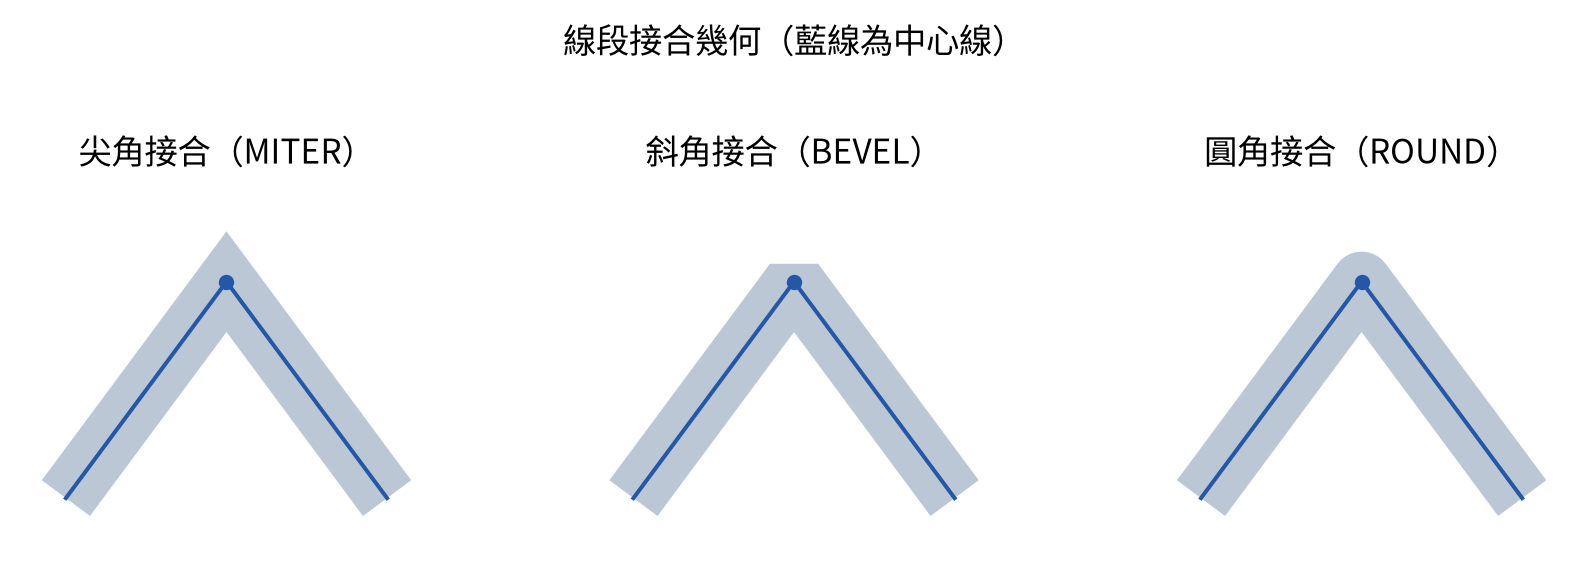
\includegraphics[width=\linewidth]{docs/figures/ch04_stroke-join.png}
        \caption{Miter、Bevel、Round Join}
        \label{fig:stroke-join}
    \end{subfigure}\hfill
    \begin{subfigure}[t]{.41\textwidth}
        \centering
        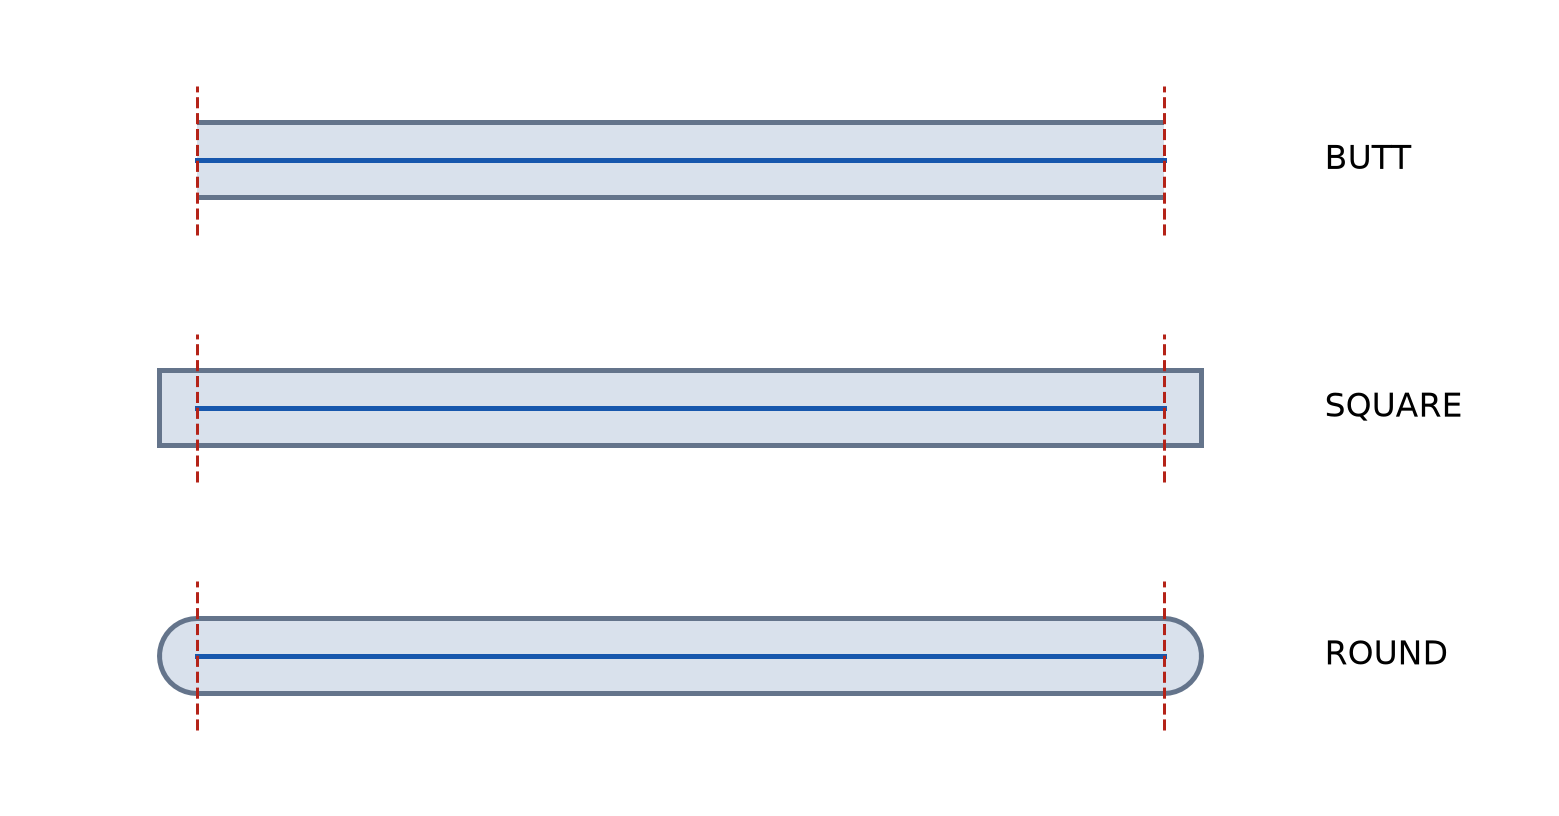
\includegraphics[width=\linewidth]{docs/figures/ch04_stroke-cap.png}
        \caption{Butt、Square、Round Cap}
        \label{fig:stroke-cap}
    \end{subfigure}
    \caption{程式支援的 Line Join 與 Line Cap}
    \label{fig:stroke-join-cap}
\end{figure}

\subsection{Line Cap}
\label{sec:line-cap}

開放路徑的第一點沒有前一點、最後一點沒有下一點，程式將缺少的鄰點設為頂點本身。這兩個頂點只有一個方向，因此不計算 Join，改依設定繪製 Cap。圖~\ref{fig:stroke-cap} 的紅色虛線為原始端點位置，三種 Cap 的差別如下：
\begin{itemize}
    \item \textbf{Butt}：截面 $B\pm h\vec n$ 即為線身盡頭，邊界停在端點上。
    \item \textbf{Square}：將端點截面沿線段方向向外推 $h$，起點朝 $-\vec v$、終點朝 $+\vec u$。由於只移動線身四邊形的頂點，延伸部分不需額外三角形。
    \item \textbf{Round}：以端點為圓心、$h$ 為半徑，從截面一側至另一側繪製半圓 triangle fan；起點的半圓位於線段後方，終點的半圓位於前方。
\end{itemize}

封閉路徑（Rectangle、Ellipse、Polygon）取鄰點時首尾相接，第一點的前一點即為最後一點，因此每個頂點都套用 Join，不會出現 Cap。若路徑只有一個頂點（例如 Pencil 僅點擊一次），則直接依 Cap 繪製：Round 為直徑 $w$ 的圓點，Square 為邊長 $w$ 的正方形，Butt 不繪製任何內容。

\subsection{Miter Limit}
\label{sec:miter-limit}

Miter 在很尖的轉角會拉得很長。設中心線夾角為 $\theta$、半線寬為 $h$，原頂點至 Miter 尖端的距離為 $m$。角平分線會把夾角分成 $\theta/2$，而 offset 邊界至中心線的垂直距離正好是 $h$，因此由直角三角形可得
\[
    \sin\!\left(\frac{\theta}{2}\right)=\frac{h}{m},
    \qquad
    m=\frac{h}{\sin(\theta/2)}.
\]
Miter Limit $L$ 定義為允許的最大 Miter 長度與半線寬之比，所以條件為
\[
    \frac{m}{h}\le L.
\]
代入前式後可得到
\[
    \frac{1}{\sin(\theta/2)}\le L
    \quad\Longleftrightarrow\quad
    \theta\ge 2\arcsin\!\left(\frac{1}{L}\right).
\]
因此 $L$ 越大，允許的最小夾角越小，Miter 也可能拉得越長。程式預設 $L=4$，對應的最小夾角約為 $29^\circ$；不符合條件時改用 Bevel，避免出現過長尖刺。

\begin{figure}[htbp]
    \centering
    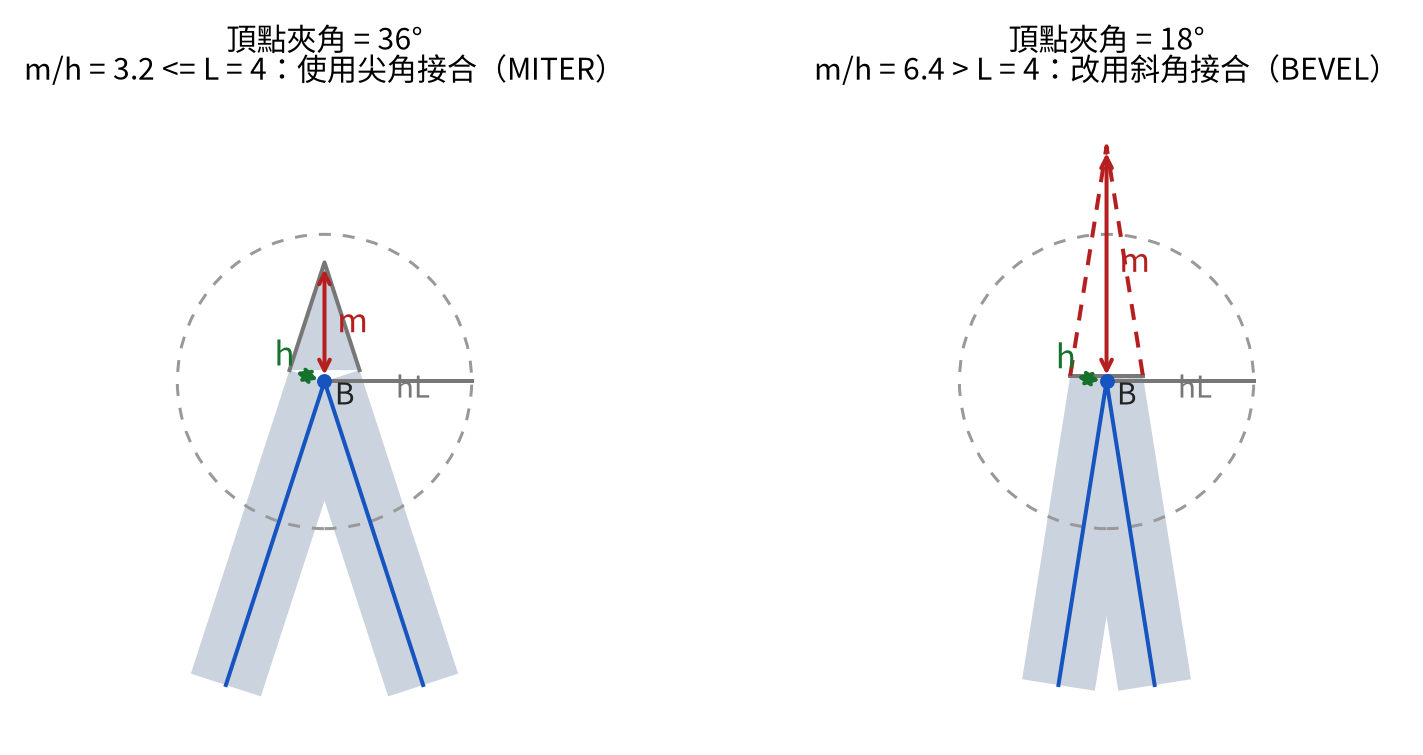
\includegraphics[width=.62\textwidth]{docs/figures/ch04_miter-limit.png}
    \caption{Miter 長度在限制內與超過限制時的處理}
    \label{fig:miter-limit}
\end{figure}

\subsection{退化幾何處理}
\label{sec:stroke-degenerate}

第~\ref{sec:line-join} 節的做法假設每個頂點前後兩段都有明確方向，且轉角夾角合理。實際以 Pencil 繪製時，路徑經常出現重複點、極短線段、幾乎共線或接近 $180^\circ$ 的折返。這些情況下，單位方向或 offset line 交點在數值上不穩定，若直接套用一般公式，容易產生跨越畫面的尖刺或錯誤的三角形，因此程式針對以下三種情況另外處理。

\paragraph{重複點與零長度線段}
零長度線段沒有方向，無法計算法向量。第~\ref{sec:pencil-sampling} 節的取樣距離已在輸入階段避免大部分過近的點；繪製前，程式再移除與前一點座標差小於 $\eps$ 的連續重複點。之後若頂點與前一點或下一點仍重合，就視為該側沒有線段：不產生線身，也不計算 Join，與第~\ref{sec:line-cap} 節的端點採用相同處理。

\paragraph{近平行與折返}
當 $\abs{c}\le\eps$ 時，兩段幾乎平行，offset line 交點不存在或極不穩定，此時改以內積 $d=\vec u\cdot\vec v$ 區分兩種情況：
\begin{itemize}
    \item \textbf{$d>0$，幾乎同方向}：頂點實際上沒有轉彎，不需要 Join。$\vec n_0$ 與 $\vec n_1$ 理論上相同，程式取兩段截面點的平均值作為共用截面，以減少浮點誤差造成的細縫。
    \item \textbf{$d<0$，接近 $180^\circ$ 折返}：路徑原地掉頭，內側與外側的概念已經退化，Miter 交點也不存在。程式以頂點 $B$ 作為內側點，以進入線段在 $B$ 的兩個截面端點作為外側點，設定為 Round 時補上半圓，否則一律使用 Bevel，使折返處成為平整或圓弧的端面。
\end{itemize}
另外，即使 $\abs{c}>\eps$，若 offset line 求交仍因數值問題失敗，程式同樣改用 Bevel 或 Round，並以 $B$ 作為內側點。

\paragraph{內側交點過遠}
第~\ref{sec:miter-limit} 節的 Miter Limit 只限制外側交點。內側交點與頂點的距離同樣是 $h/\sin(\theta/2)$，轉角越尖就越遠；若相鄰線段很短，內側交點甚至會落在線段範圍之外，此時把內側邊界收到該點，三角形會翻折並向外突出。因此程式以
\[
    \norm{X_{\text{in}}-B}\le\max\!\left(2h,\ \min(\ell_{AB},\ell_{BC})+h\right)
\]
作為內側交點的合理範圍，其中 $\ell_{AB}$、$\ell_{BC}$ 為前後兩段的長度。超出範圍時改以頂點 $B$ 作為內側點，雖然內側會有少量重疊，但能避免短線段產生延伸到畫面遠處的三角形。
